% \acresetall
\chapter{Clinical background}\label{chap:clinical-background}
\begin{flushright}{\slshape 
        What, so everyone’s supposed to sleep every single night now? You realize that nighttime makes up half of all time?} \\ \medskip
        --- Rick Sanchez\\Rick and Morty, season 1, pilot episode
\end{flushright}
\vspace{6cm}
    
    This chapter aims to provide the reader with a basic and preliminary understanding of sleep science. 
    First, the fundamental aspects of sleep as a physiological phenomenon are reviewed. Unless otherwise stated, the context will be concerning sleep in primarily healthy adults. 
    This will be followed by a description of how sleep is recorded, quantified and analyzed in clinical practice.
    The chapter will conclude with a section on some of the major challenges and difficulties that arise in clinical sleep practice, such as inter- and intra-rater variability, and how this can affect clinical outcomes.
    
    \section{Fundamental aspects of sleep}\label{sec:fundamental-aspects-sleep}
    
        Sleep is ubiquitous to human life. 
        Our bodies might seem static, but sleep is actually a complex, physiological state comprised of multiple, dynamic processes, that are observable across multiple recording modalities. 
        But although we spend almost a third of our lifetime sleeping, there are still many aspects that are unknown to science. 
       
       The general understanding of how our sleep is structured includes two concepts important for this thesis: sleep architecture and sleep events.
        \begin{description}
            \item[Sleep architecture] refers to the structure of sleep, how it is divided into different states based on physiological characteristics, and the dynamics of those states across the night.
            This can also be called \textit{macro-sleep}, as it concerns the overall macro-structure of our sleep patterns.
            \item[Sleep events] are discrete observations with various characteristics that are distinct for the specific event type.
            Many such events can happen during sleep, and the duration and scope of these events can vary from short and localized (leg movements, sleep spindles), to long and broad (arousals, apneas).
            The description and characterization of these events can also be called \textit{micro-sleep}, but this term is also sometimes applied to sleep architecture on a small time-scale.
            In this thesis, I will refer to this concept as either \textit{micro-sleep events} or just \textit{sleep events} for short.
        \end{description}
        
        \subsection{Sleep architecture}\label{sec:sleep-architecture}
            On average, normal sleep in adult humans lasts between 7-9 hours per night with substantial variability between persons. 
            During this period, the brain and body cycle between alternating \textit{sleep stages}, which can be categorized into a state of drowsiness or semi-conscious \ac{W}, a \ac{REM} sleep stage, and three \ac{NREM} stages, \ac{N1}, \ac{N2}, and \ac{N3}.
            The main distinction between sleep stages comes from the amplitude and spectral content of the brain signals as measured using \ac{EEG}. 
            For example, wakefulness and \ac{REM} sleep are associated with high frequency, low amplitude content such as theta or alpha rhythm activity, while the \ac{NREM} sleep stages are associated with low frequency, high amplitude content in the delta rhythm range. 
            
            However, certain brain stages are also characterized by the presence of certain micro-structure events with very distinct morphologies, such as sleep spindles or K-complexes in the \ac{EEG}, or \acp{REM} which are recorded with \ac{EOG}~\citep{Brown2012, Saper2010, Carskadon2011}. 
            Muscle activity, which is typically recorded using \ac{EMG} of the submentalis\graffito{The submentalis is located below the chin, while the anterior tibialis is located on the shin.} and anterior tibialis muscles, can also be used to distinguish between sleep stages.
            
            \begin{table}
            \small
            % \setcitestyle{super}
            % \begin{adjustwidth*}{}{-\marginparwidth-\marginparsep}
            \centering
            \begin{threeparttable}
                \caption[Clinical \acs{EEG} frequency bands]{Clinical \acs{EEG} frequency bands.}
                \label{tab:eeg_rythms}
                \begin{tabular}{@{}lcc@{}} \toprule
                % \begin{tabular}{lc}\toprule
                    \textbf{Rhythm} & \textbf{\citet{Brown2012}} & \textbf{\acs{AASM}2020~\cite{Berry2020}} \\ \midrule
                    Delta & \SIrange{1}{4}{\hertz} & \SIrange{0}{3.99}{\hertz} \\
                    Theta & \SIrange{4}{8}{\hertz} & \SIrange{4}{7.99}{\hertz} \\
                    Alpha & \SIrange{8}{14}{\hertz} & \SIrange{8}{13}{\hertz} \\
                    Beta & \SIrange{15}{30}{\hertz} & $>\SI{13}{\hertz}$\\
                    Gamma & \SIrange{30}{120}{\hertz} & n.d.\\ \midrule
                    \acs{SWA} & \SIrange{0.5}{4}{\hertz} & \SIrange{0.5}{2.0}{\hertz} \\
                    \acs{LAMF} & n.d. & \SIrange{4}{7}{\hertz} \\\bottomrule
                \end{tabular}
                \begin{tablenotes}
                    \item n.d., not defined; %
                    \describe{EEG}; %
                    \describe{SWA}; %
                    \describe{LAMF}.
                \end{tablenotes}
            \end{threeparttable}
            % \end{adjustwidth*}
            \end{table}
            
            \begin{figure}[htp]
            \begin{adjustwidth*}{}{-\marginparwidth-\marginparsep}
                \centering
                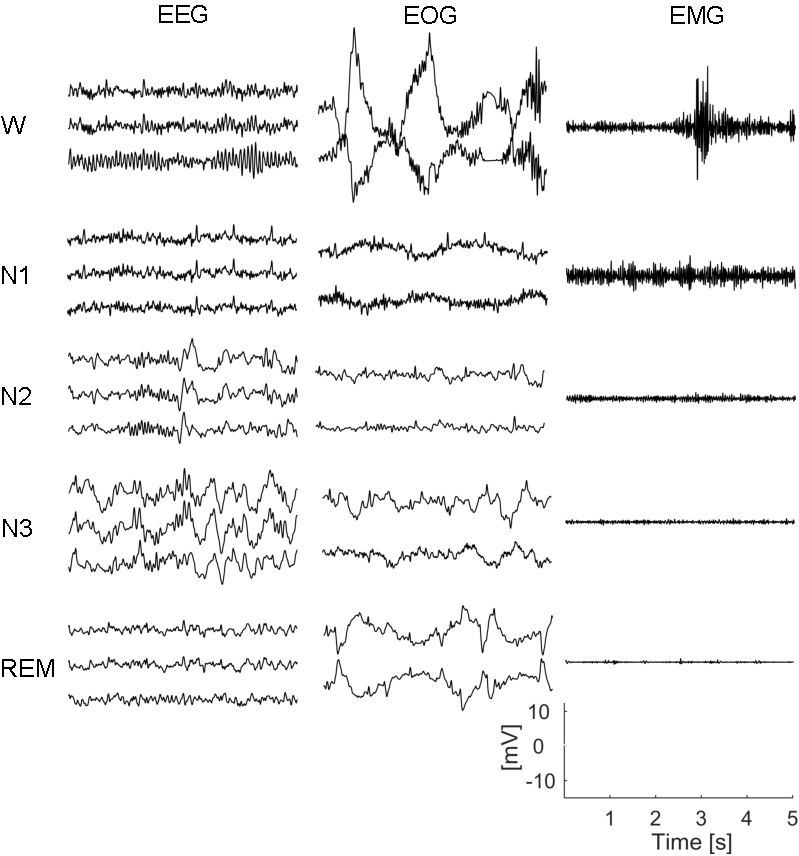
\includegraphics[width=\linewidth]{figures/clinical-background/TypicalWaves.pdf}
                \caption[Signal content in different sleep stages]{Typical waveforms encountered in different sleep stages. The left column displays the progression from low amplitude, mixed frequency content such as alpha rhythms in \acs{W}, towards low frequency, high amplitude delta rhythms in the deep \acs{N3} sleep. In the middle is shown \acsp{REM} and reading eye movements in \acs{W}, and \acsp{SEM} or no activity in \acs{NREM} stages. Due to their proximity to the frontal area, delta rhytms might be visible in the \acs{EOG} during \acs{N3}. The right-most column shows the \acs{EMG} amplitude progression from high in \acs{W} to low in \acs{N3}. The bottom row shows the paradoxical nature of \acs{REM} sleep with \acs{LAMF} content and theta rhythms in the \acs{EEG}, \acsp{REM}  in the \acs{EOG}, and atonia in the \acs{EMG}. Reprinted with permission from~\cite{Cesari2019}.}
                \label{fig:clinical-background:stage-specifics}
            \end{adjustwidth*}
            \end{figure}
            
            The following sections review the major electrophysiological characteristics for the five sleep stages currently defined by the~\ac{AASM}, which is summarized in~\cref{tab:stage-characteristics}. 
            A graphical overview of typical signal content in the \ac{EEG}, \ac{EOG} and \ac{EMG} for the five sleep stages is shown in~\cref{fig:clinical-background:stage-specifics}.
            
            \subsubsection{Wakefulness}\label{sec:wakefulness}
            Spanning from a full awareness state to a quiet awakening or drowsiness state, this stage generally accounts for about \SI{5}{\percent} of the total time in bed from lights out to lights on in healthy adults.
            In this stage, the brain typically exhibits low amplitude, high\graffito{\ac{EEG} rhythms in the alpha range or higher.} frequency content in small areas and more wide-spread theta rhythms.
            During quiet awakening, these theta rhythms increase in the frontal area of the brain, while alpha rhythms are dominant over the occipital region, especially when the eyes are closed.
            With eyes open, this stage is characterized by eye blinking, reading eye movements and \acp{REM}.
            The chin muscle tone is typically high with unspecific amplitude.
            
            \begin{table}
                \small
                \centering
                \caption[Sleep stage characteristics]{Sleep stage characteristics according to \acs{AASM}2020~\cite{Berry2020}.}
                \label{tab:stage-characteristics}
                \begin{threeparttable}
                \begin{tabular}{@{}ll@{}} \toprule
                    \textbf{Sleep stage} & \textbf{Description} \\ \midrule
                    \multirow[t]{3}{*}{\acs{W}} & \acs{EEG}: alpha (eyes closes), theta (eyes open) \\
                     & \acs{EOG}: \acsp{REM}, reading eye movements\\
                     & \acs{EMG}: high, but variable, amplitude \\ \midrule
                    \multirow[t]{3}{*}{\ac{N1}} & \acs{EEG}: \acs{LAMF} content, theta rhythms \\ 
                     & \acs{EOG}: \acsp{SEM}\\
                     & \acs{EMG}: variable amplitude, usually lower than in \acs{W}\\ \midrule
                    \multirow[t]{3}{*}{\ac{N2}} & \acs{EEG}: K-complexes, sleep spindles  \\
                     & \acs{EOG}: No activity, or \acsp{SEM} \\
                     & \acs{EMG}: variable amplitude, usually lower than in \acs{N1} \\ \midrule
                    \multirow[t]{3}{*}{\ac{N3}} & \acs{EEG}: \acs{SWA}, large amplitude delta rhythms \\
                     & \acs{EOG}: No activity, or \acsp{SEM} \\
                     & \acs{EMG}: variable amplitude, usually lower than in \acs{N2} \\ \midrule
                    \multirow[t]{3}{*}{\ac{REM}} & \acs{EEG}: \acs{LAMF} content, theta rhythms, sawtooth waves, \acs{PGO} waves\\
                     & \acs{EOG}: \acp{REM}\\
                     & \acs{EMG}: muscle atonia, phasic bursts\\ \bottomrule
                \end{tabular}
                \begin{tablenotes}[para,flushleft]
                    \item \describe{LAMF}; %
                    \describe{PGO}; %
                    \describe{REM}; %
                    \describe{SEM}.
                \end{tablenotes}
                \end{threeparttable}
            \end{table}
            
            \subsubsection{NREM sleep}
            Sleep in humans generally commences when a person progresses from \ac{W} to one of the three stages of \ac{NREM}\graffito{Up until 2007, \ac{NREM} sleep was divided in four stages: S1, S2, S3, and S4 (slow wave sleep). The latter two was merged in \ac{AASM}2007 into \ac{N3}.}.
            They generally constitute approximately \SIrange{2}{5}{\percent}, \SIrange{45}{55}{\percent}, and \SIrange{13}{23}{\percent} of the \ac{TST} for the first, second, and third \ac{NREM} stage, respectively.
            The order of \ac{N1}, \ac{N2}, and \ac{N3} represents a continuum of the depth of sleep, which is primarily constituted by a progressive slowing of the \ac{EEG} activity from low amplitude, high frequency alpha and theta rhythms, to low frequency delta rhythms with large amplitude.
            Furthermore, another major indicator of deepening sleep is the increasing arousal thresholds associated with the progression from \ac{N1} to \ac{N3}~\cite{Brown2012, Carskadon2011}.
            
            \paragraph{N1} This is the first stage encountered during normal sleep, and is generally considered to be a transitional stage between drowsiness, or lighter sleep, and deeper sleep.
            It is characterized by mixed frequency content, as the alpha rhythms are progressively reduced and replaced with theta rhythms.
            Additionally, small sleep events called \textit{vertex sharp waves} also appear in the \ac{EEG} during this stage\graffito{Vertex sharp waves are sharply contoured waveforms with a very short duration of less than \SI{0.5}{\second}}.
            \Acp{REM} and reading eye movements are replaced with slow eye movements and the muscle tone is reduced compared to \ac{W}.
            
            \paragraph{N2} Although theta rhythms from \ac{N1} continue, brain activity in \ac{N2} exhibits discrete sleep events like \textit{sleep spindles} and \textit{K-complexes}.\graffito{These events will be described in~\cref{sec:sleep-events}}
            Eye movement activity is not typically seen in this stage, while muscle activity is further reduced from that of \ac{N1}.
            
            \paragraph{N3} The last of the three \ac{NREM}, the \ac{N3} stage is also known as \textit{deep sleep}.
            In this stage, the \ac{EEG} content shifts towards more pronounced delta wave activity, especially \ac{SWA} larger than \SI{75}{\micro\volt} in the frontal regions.
            Eye movement activity is typically not seen, but \ac{SWA} intrusion artifacts from the frontal \ac{EEG} can sometimes be seen.
            The muscle activity is low, and the muscle tone typically has an amplitude between that of \ac{N2} and \ac{REM}.
            
            \subsubsection{REM sleep}
            The defining characteristic of this stage of sleep is the appearance of \ac{REM}\graffito{Conjugate, irregular, sharply peaked eye movements with an initial deflection lasting less than \SI{500}{\milli\second}~\cite{Berry2020}} activity observed in the \ac{EOG}, desynchronized \ac{LAMF} \ac{EEG} activity, and suppression of skeletal muscle activity (atonia) due to brainstem-mediated inhibition of the alpha motor-neurons~\cite{Carskadon2011,Simor2020}.    
            This stage typically accounts for \SIrange{20}{25}{\percent} of the \ac{TST}~\cite{Carskadon2011}, and is associated with the majority of dreaming activity, although evidence suggests dreaming also occurs in \ac{NREM}~\cite{Foulkes1962, Hobson2009, McNamara2010, Brown2012, Simor2020}, albeit at a less vivid level~\cite{Siclari2017}.
            
            Some studies indicate that \ac{REM} sleep is comprised of two distinct micro-states~\cite{Simor2020}: a \emph{phasic} state characterized by the appearance of \ac{PGO} and \emph{sawtooth} waves\graffito{Characteristic 2-4 Hz rhythmic oscillations during \ac{REM} sleep that have a triangular shape and maximal amplitude at frontal and central derivations.}, \acp{REM} and muscle twitches~\cite{Takahara2009}; and a \emph{tonic} state in between phasic states that is characterized by \ac{LAMF} and theta rhythms, and a higher arousal threshold~\cite{Ermis2010}.
            Studies on the effects of auditory stimulation and event related potentials in \ac{REM} microstates confirm the heterogeneity of \ac{REM} sleep~\cite{Sallinen1996,Takahara2002,Takahara2006}. This is underlined by clinical studies on \ac{RBD} patients, which suggest a distinction in the level of activation of the sensory motor system during tonic and phasic \ac{REM}~\cite{Manni2009,DeCarli2016,Sunwoo2019}.
            
            \begin{figure}[tb]
                \begin{adjustwidth*}{}{-\marginparwidth-\marginparsep}
                \centering
                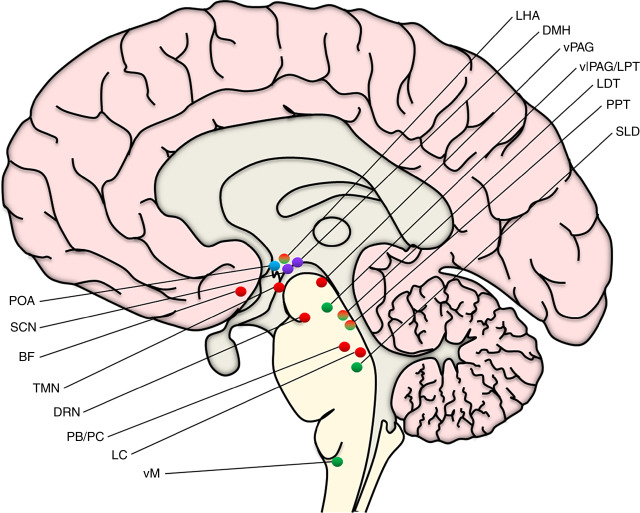
\includegraphics[width=\textwidth]{figures/clinical-background/AnatomyPhysiologySleep/Figure1_1.jpg}
                \caption[Brain centers involved in sleep-wake control.]{%
                Locations of the brain centers involved in sleep-wake control. %
                The predominant role of each center is color-coded: red for arousal, blue for sleep, green for \ac{REM} sleep, purple for circadian regulation, and multicolored for mixed activity. %
                \describe{BF}; %
                \describe{DMH}; %
                \describe{DRN}; %
                \describe{LC}; %
                \describe{LDT}; %
                \describe{LHA}; %
                \describe{LPT}; %
                \describe{PB}; %
                \describe{PC}; %
                \describe{POA}; %
                \describe{PPT}; %
                \describe{SCN}; %
                \describe{SLD}
                \describe{TMN}; %
                \describe{vM}; %
                \describe{vlPAG}; %
                \describe{vPAG}. %
                Reprinted from~\cite{Schneider2017} with permission from Elsevier.}
                \label{fig:clinical-background:sleep-wake-control}
                \end{adjustwidth*}
            \end{figure}
            
            
        \subsection{Neurobiological control of sleep}\label{sec:control-sleep}
            
            % \begin{figure}
            %     \centering
            %     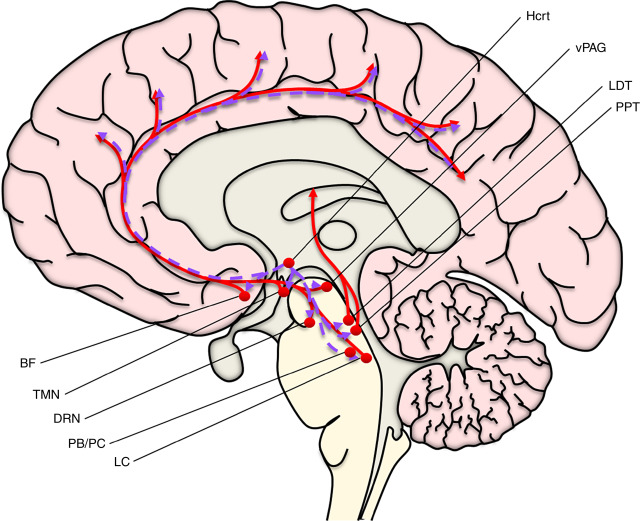
\includegraphics[width=\textwidth]{figures/clinical-background/AnatomyPhysiologySleep/Figure1_3.jpg}
            %     \caption[Arousal-promoting pathways.]{%
            %     Arousal-promoting pathways.%
            %     \describe{BF}; %
            %     \describe{DRN}; %
            %     \describe{hcrt}; %
            %     \describe{LC}; %
            %     \describe{LDT}; %
            %     \describe{PB}; %
            %     \describe{PC}; %
            %     \describe{PPT}; %
            %     \describe{TMN}; %
            %     \describe{vPAG}. %
            %     Reprinted from~\cite{Schneider2017} with permission from Elsevier.}
            %     \label{fig:clinical-background:arousal-pathways}
            % \end{figure}
            
            \subsubsection{The wake-sleep switch}
            
            The \textit{wake-sleep switch} consists of several neuronal populations in the areas of the upper brainstem, hypothalamic, and forebrain responsible for promoting wakefulness and sleep, as shown in~\cref{fig:clinical-background:wake-sleep-switch}~\cite{Saper2010}.
            
            Two major pathways promoting wakefulness are located in the upper brainstem.
            \cref{fig:clinical-background:wake-sleep-switch}\textsc{\textsf{a}} shows cholinergic neurons (cyan) \ac{PPT} projecting to the thalamus, \ac{LHA}, and \ac{BF} from the \ac{LDT}, thereby driving extensive cortical activation. The monoaminergic and glutaminergic neurons (green) in the \ac{LC}, \ac{PB}, \ac{PC}, \ac{DRN}, \ac{vPAG}, and \ac{TMN} project to the forebrain, cerebral cortex, thalamic and hypothalamic areas.
            A special population of neurons in the \ac{LHA} promotes wakefulness by directly exciting both wakefulness pathways as well as the \ac{BF} and cerebral cortex by secreting \ac{hcrt}\graffito{Two research teams simultaneously discovered these neuropeptides and gave them the names hypocretin and orexin, respectively.}~\cite{Peyron1998}.
            
            The main pathway for sleep promotion, shown in purple in~\cref{fig:clinical-background:wake-sleep-switch}\textsc{\textsf{b}}, originates in neurons in the \ac{VLPO} and \ac{MnPO} areas of the hypothalamus and inhibits the pathways promoting wakefulness.
            In turn, these pathways can likewise inhibit the sleep-promoting activity in the \ac{VLPO} and \ac{MnPO} areas, as shown in~\cref{fig:clinical-background:wake-sleep-switch}\textsc{\textsf{c}}.
            
            This mutual inhibitory activity is the basis for the wake-sleep switch acting like an electronic switch.
            When one group of neurons gains a slight advantage over the other, a rapid decrease in neuronal firing activity on the losing side ensures a fast and complete transition between the two states~\cite{Saper2010, Schneider2017}.
            
            \begin{figure}
                % \centering
                \begin{adjustwidth*}{}{-\marginparwidth-\marginparsep}
                \centering
                % 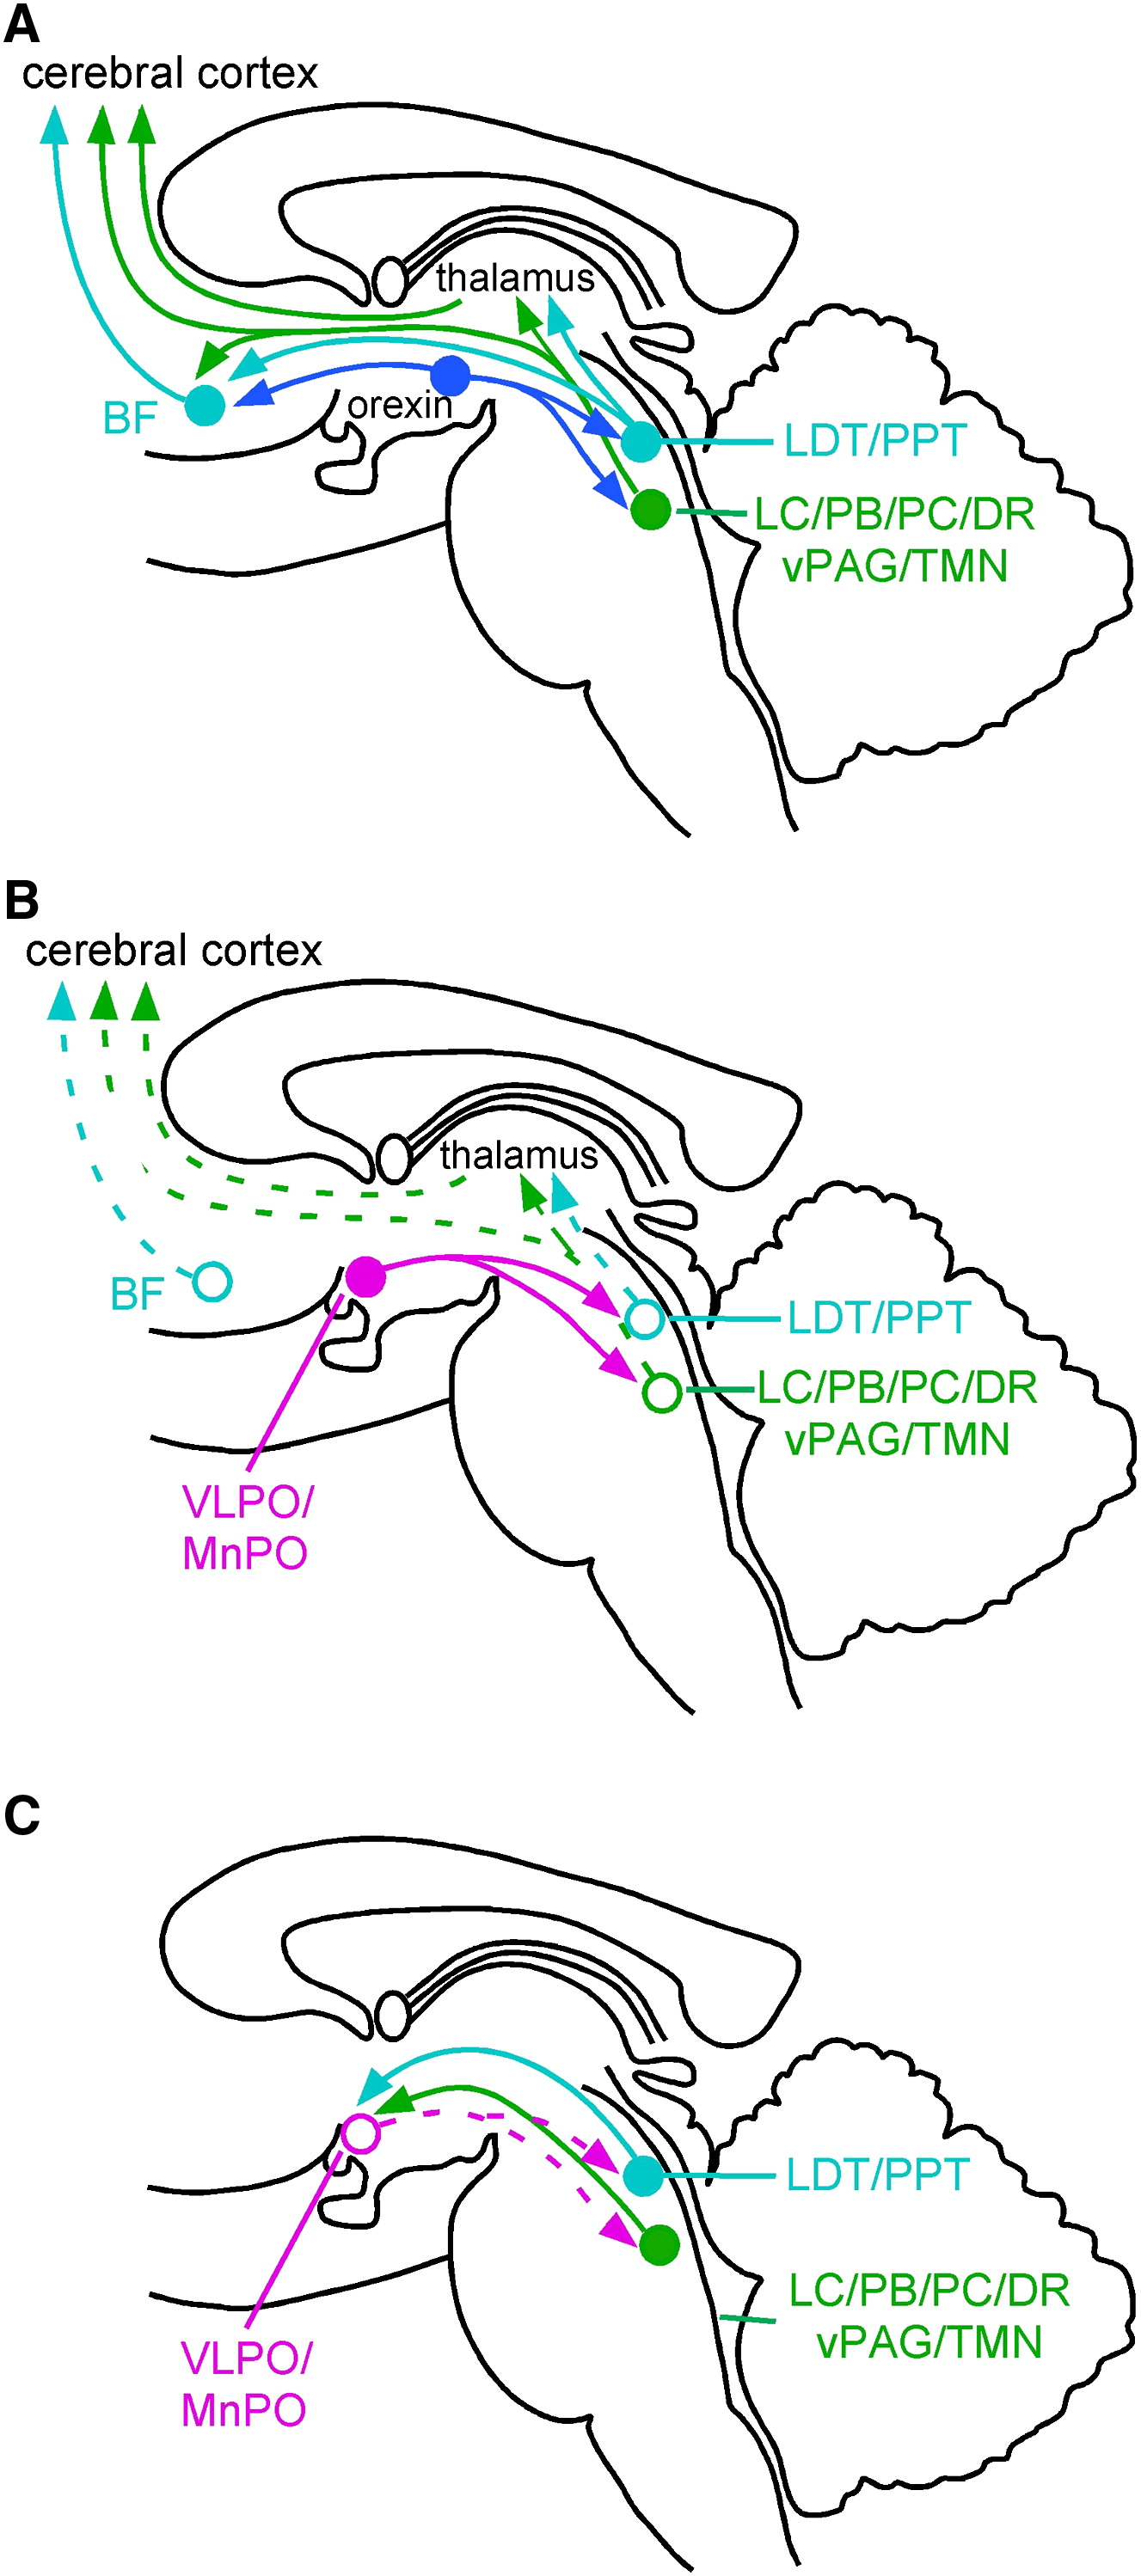
\includegraphics[width=\textwidth]{figures/clinical-background/SleepStateSwitching/Figure1.png}
                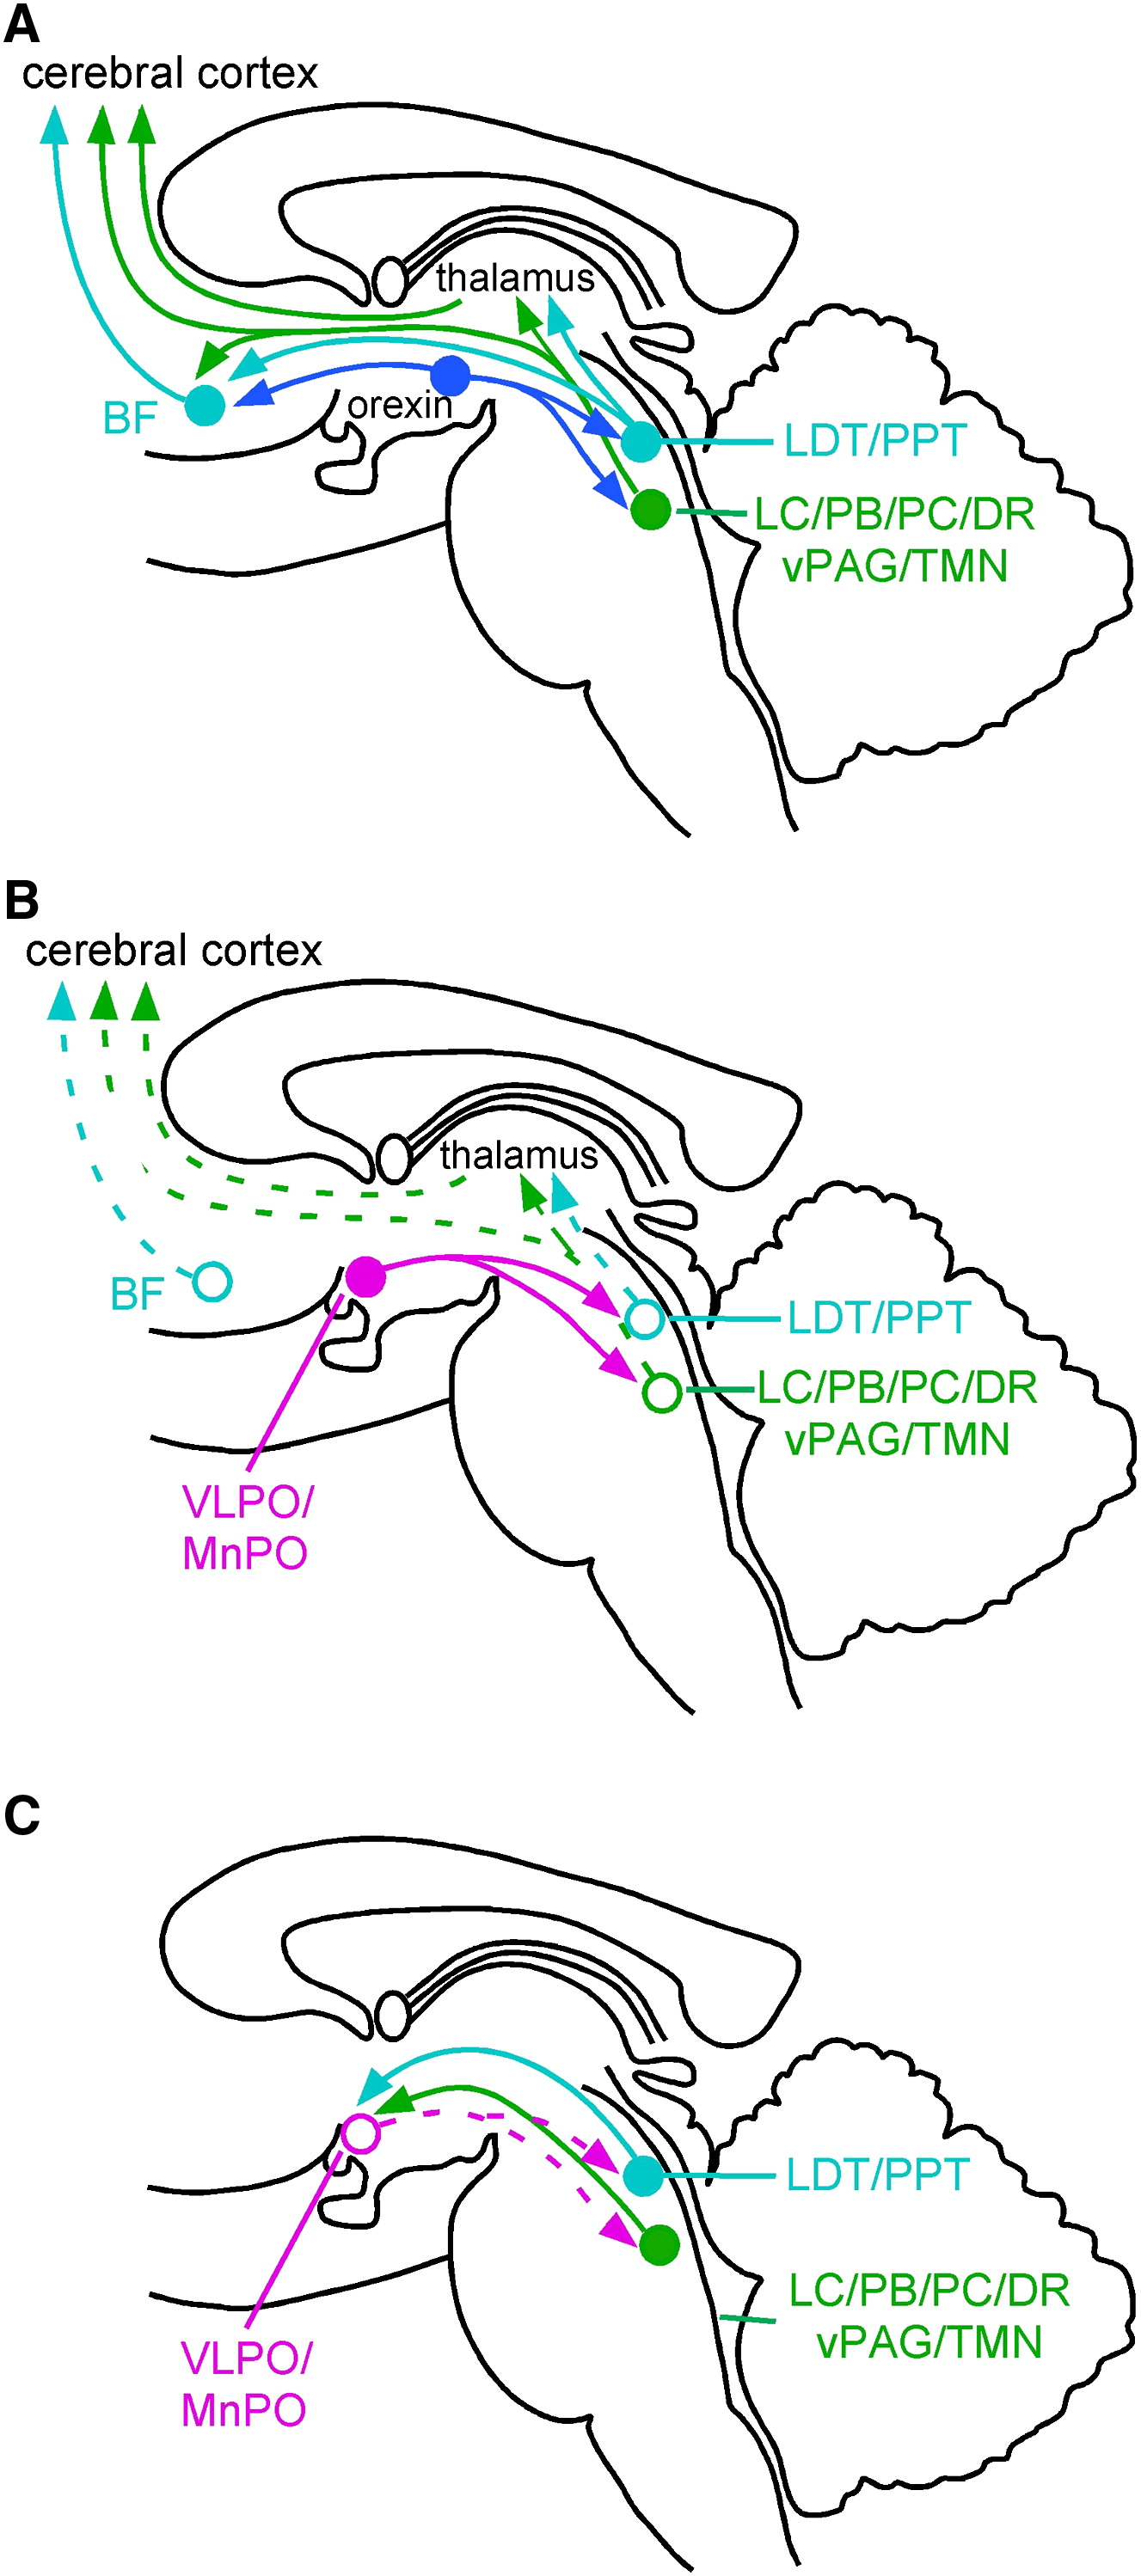
\includegraphics[height=0.775\textheight]{figures/clinical-background/SleepStateSwitching/Figure1.png}
                \caption[Structures involved in the wake-sleep switch]{%
                Structures involved in the wake-sleep switch. %
                \begin{enumerate*}[label=\textbf{\textsf{\Alph*}}]
                    \item The two main wake-promoting pathways originating in the upper brainstem. Cholinergic neurons (aqua) in the \acs{LDT} and \acs{PPT} project to the thalamus and \acs{BF}, while predominantly monoaminergic neurons (green) in the \acs{LC}, \acs{PB}, \acs{PC}, \textsc{dr}, \acs{vPAG}, and \acs{TMN} project directly to the hypothalamus, \acs{BF} and cerebral cortex. Hypocretin-producing neurons in the hypothalamus reinforce activation in both pathways, while directly innervating the \ac{BF}.
                    \item The main sleep-promoting pathways originate in the \acs{VLPO} and \ac{MnPO} areas (purple) of the hypothalamus and inhibit the activity of the wake-promoting networks in the upper brainstem.
                    \item The wake-promoting networks in the brainstem in turn can also inhibit the activity of the sleep-promoting networks in the \acs{VLPO}/\acs{MnPO} area.
                \end{enumerate*}
                \describe{BF}; %
                \textsc{dr}: dorsal raphe; %
                \describe{LC}; %
                \describe{LDT}; %
                \describe{MnPO}; %
                \describe{PB}; %
                \describe{PC}; %
                \describe{PPT}; %
                \describe{TMN}; %
                \describe{VLPO}; %
                \describe{vPAG}. %
                Reprinted from~\cite{Saper2010} with permission from Elsevier.}
                \label{fig:clinical-background:wake-sleep-switch}
                \end{adjustwidth*}
            \end{figure}
            
            \subsubsection{The REM-NREM switch}
            
            \begin{figure}
                \begin{adjustwidth*}{}{-\marginparwidth-\marginparsep}
                \centering
                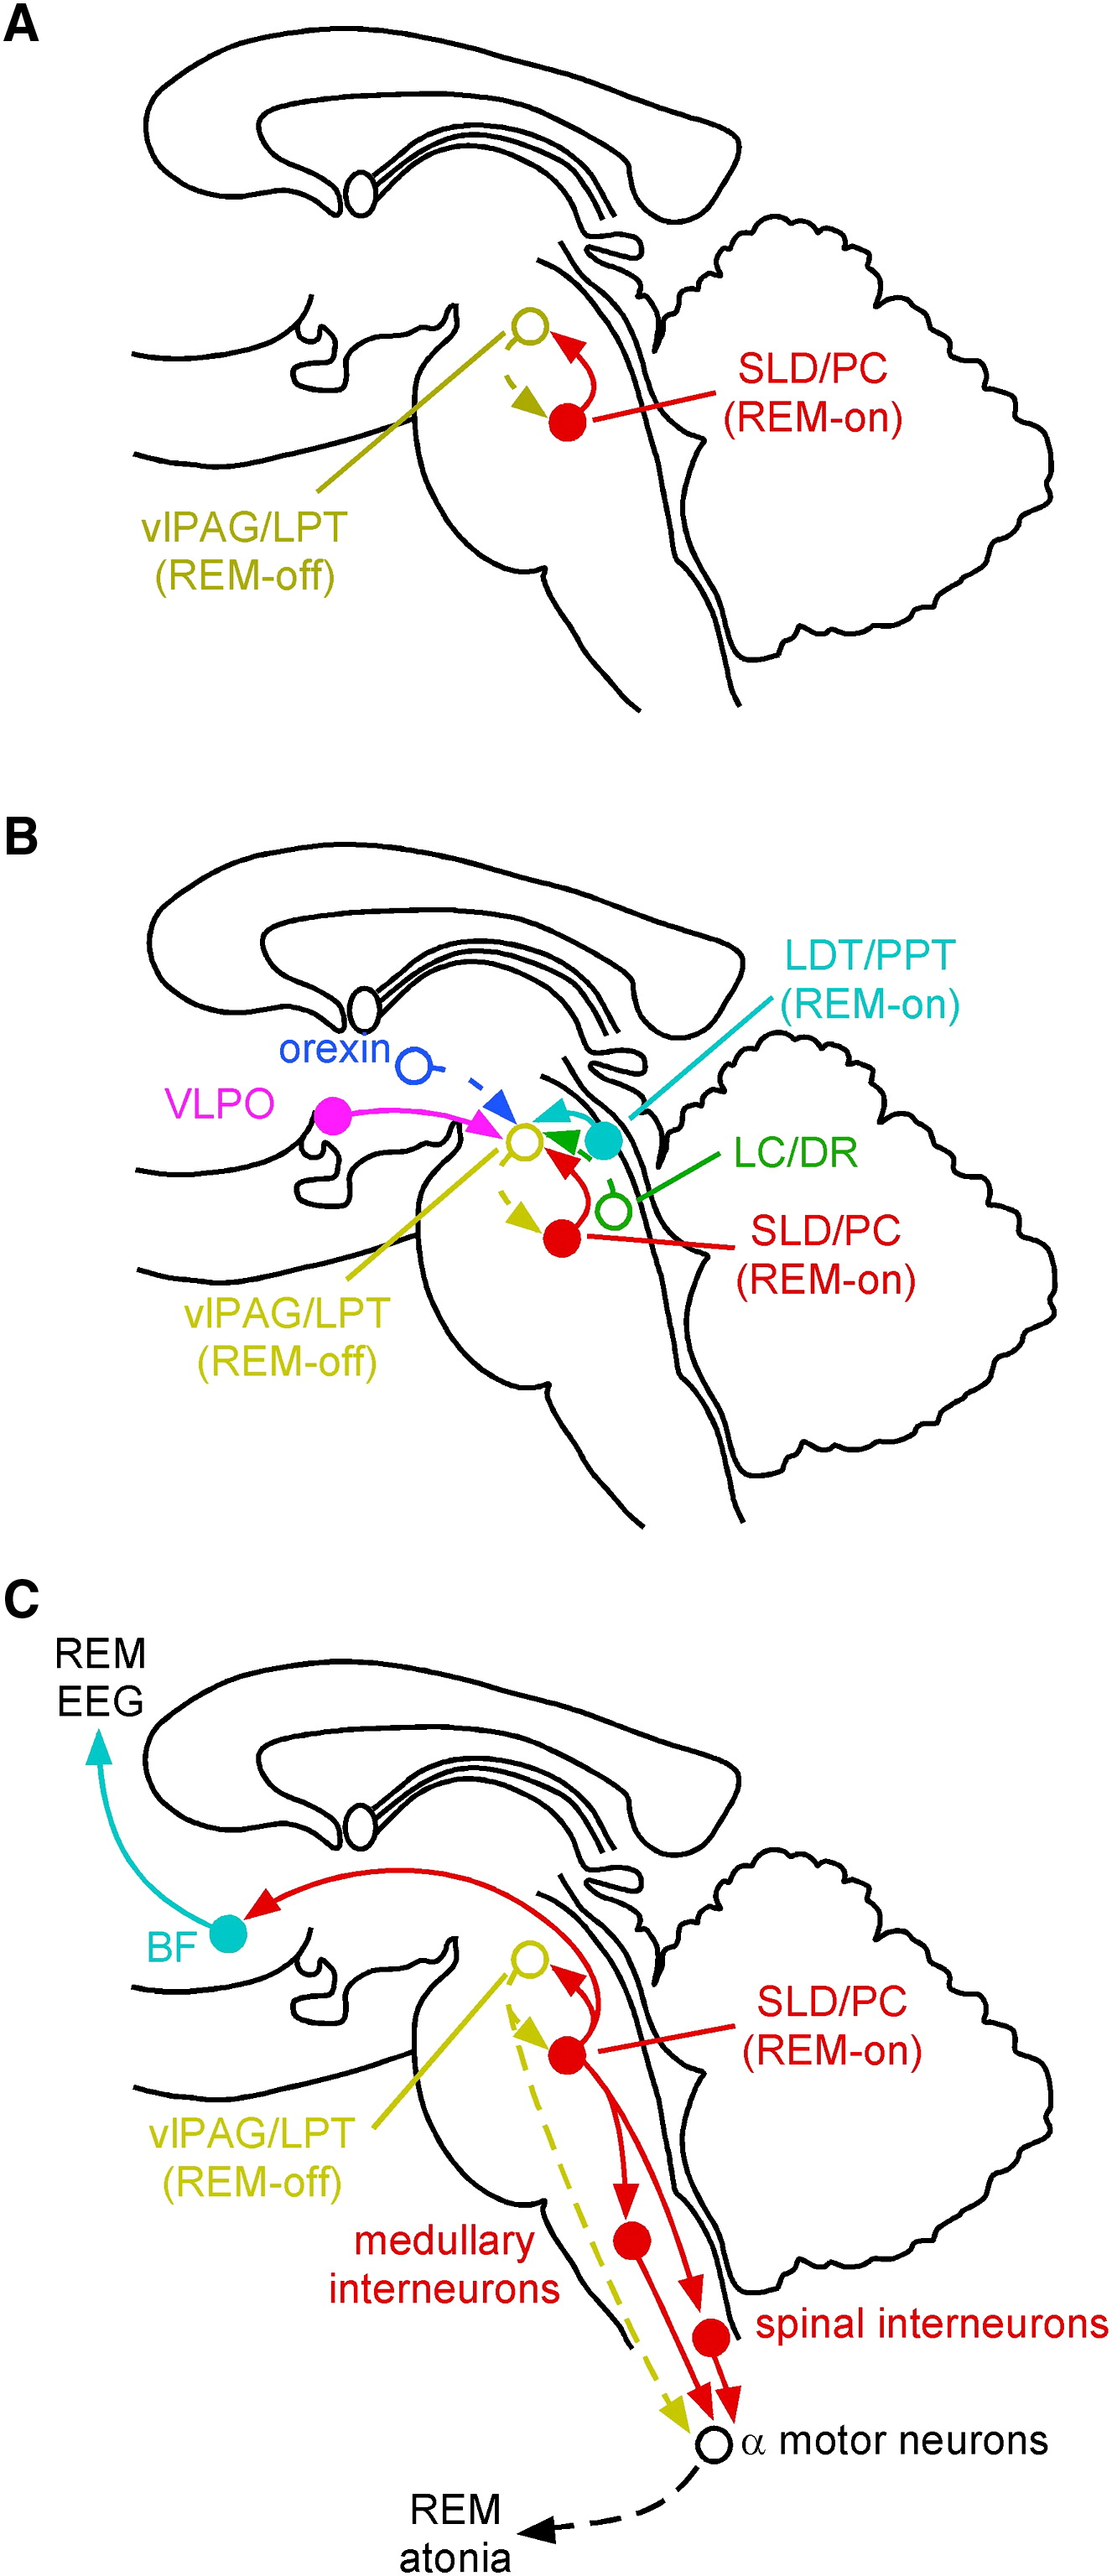
\includegraphics[height=0.775\textheight]{figures/clinical-background/SleepStateSwitching/Figure2.png}
                \caption[Structures involved in the \textsc{rem}-\textsc{nrem} switch]{%
                Structures involved in the \acs{REM}-\acs{NREM} switch. %
                \begin{enumerate*}[label=\textbf{\textsf{\Alph*}}]
                    \item Two mutually inhibitory \acs{GABA}ergic neuron groups in the brainstem form a switch for controlling transitions between \ac{REM} and \ac{NREM} sleep. Projections from the \acs{SLD} and \acs{PC} (red) promote \acs{REM}, while \acs{REM}-off projections from the \acs{vlPAG} and \acs{LPT} (gold) are most active during \ac{NREM} and thus inhibit \ac{REM}-producing activity in the \acs{SLD}/\acs{PC} nuclei.
                    \item The \acs{REM}-\acs{NREM} switch is also modulated by other neurotransmitter systems. The noradrenergic (green) neurons in the \acs{LC} and serotonergic {\scriptsize DR} inhibit \acs{REM} sleep by exciting the \acs{REM}-off neurons and inhibiting \acs{REM}-on neurons. Cholinergic (aqua) neurons in the \acs{LDT} and \acs{PPT} nuclei promote \acs{REM} sleep by the opposing actions on the same neuron groups. \acs{VLPO} neurons promote \acs{REM} sleep by inhibiting the \acs{REM}-off neurons, while orexin-producing neurons produce the opposite effect.
                    \item During \acs{REM} sleep, glutaminergic neurons in the \acs{SLD} promote \acs{REM} atonia in the skeletal muscles by way of inhibitory interneurons in the spinal cord and medulla, which act on the $\alpha$ motor neurons. Furthermore, glutamergic neurons in the \acs{PB}/\acs{PC} promote desynchronized \acs{EEG} via \acs{BF} neurons.
                \end{enumerate*}
                \describe{BF}; %
                {\scriptsize DR}: dorsal raphe; %
                \describe{LC}; %
                \describe{LDT}; %
                \describe{LPT}; %
                \describe{PC}; %
                \describe{PPT}; %
                \describe{SLD}; %
                \describe{vlPAG}; %
                \describe{VLPO}. %
                Reprinted from~\cite{Saper2010} with permission from Elsevier.}
                \label{fig:clinical-background:rem-nrem-switch}
                \end{adjustwidth*}
            \end{figure}
            
            Similar to the wake-sleep switch, the \ac{REM}-\acs{NREM} switch consists of several groups of neurons in the brainstem and hypothalamic areas, as shown in~\cref{fig:clinical-background:rem-nrem-switch}~\cite{Saper2010}.
            
            Two populations of importance, shown in~\cref{fig:clinical-background:rem-nrem-switch}\textsc{\textsf{a}}, include a group of neurons in the \ac{SLD} and \ac{PC} (red) that fires most actively during \ac{REM}, and a group in the \ac{vlPAG} and \ac{LPT} (gold) that promotes \ac{NREM} sleep by inhibiting \ac{REM}-on neurons.
            
            These two populations are acted upon by several other neurotransmitter systems as shown in~\cref{fig:clinical-background:rem-nrem-switch}\textsc{\textsf{b}}.
            One of these consists of noradrenergic neurons in the \ac{LC} and serotonergic neurons in the \ac{DRN} (green), which inhibits \ac{REM} sleep by exciting \ac{REM}-off neurons and inhibiting \ac{REM}-on neurons.
            Conversely, a system of cholinergic neurons (aqua) in the \ac{LDT} and \ac{PPT} promotes \ac{REM} sleep by the opposite mechanisms.
            Neurons in the \ac{VLPO} (purple) also promote \ac{REM} sleep by inhibiting \ac{REM}-off neurons, while \ac{hcrt}-(orexin-)producing neurons in the \ac{LHA} inhibit \ac{REM} sleep by exciting \ac{REM}-off neurons.
            
            Lastly, the glutaminergic neurons in the \ac{SLD} promote \ac{REM} atonia by exciting inhibitory interneurons in the medulla and spinal cord, as shown in~\cref{fig:clinical-background:rem-nrem-switch}\textsc{\textsf{c}}.
            
            
            \subsubsection{The flip-flop model of sleep}
            
            \begin{figure}
                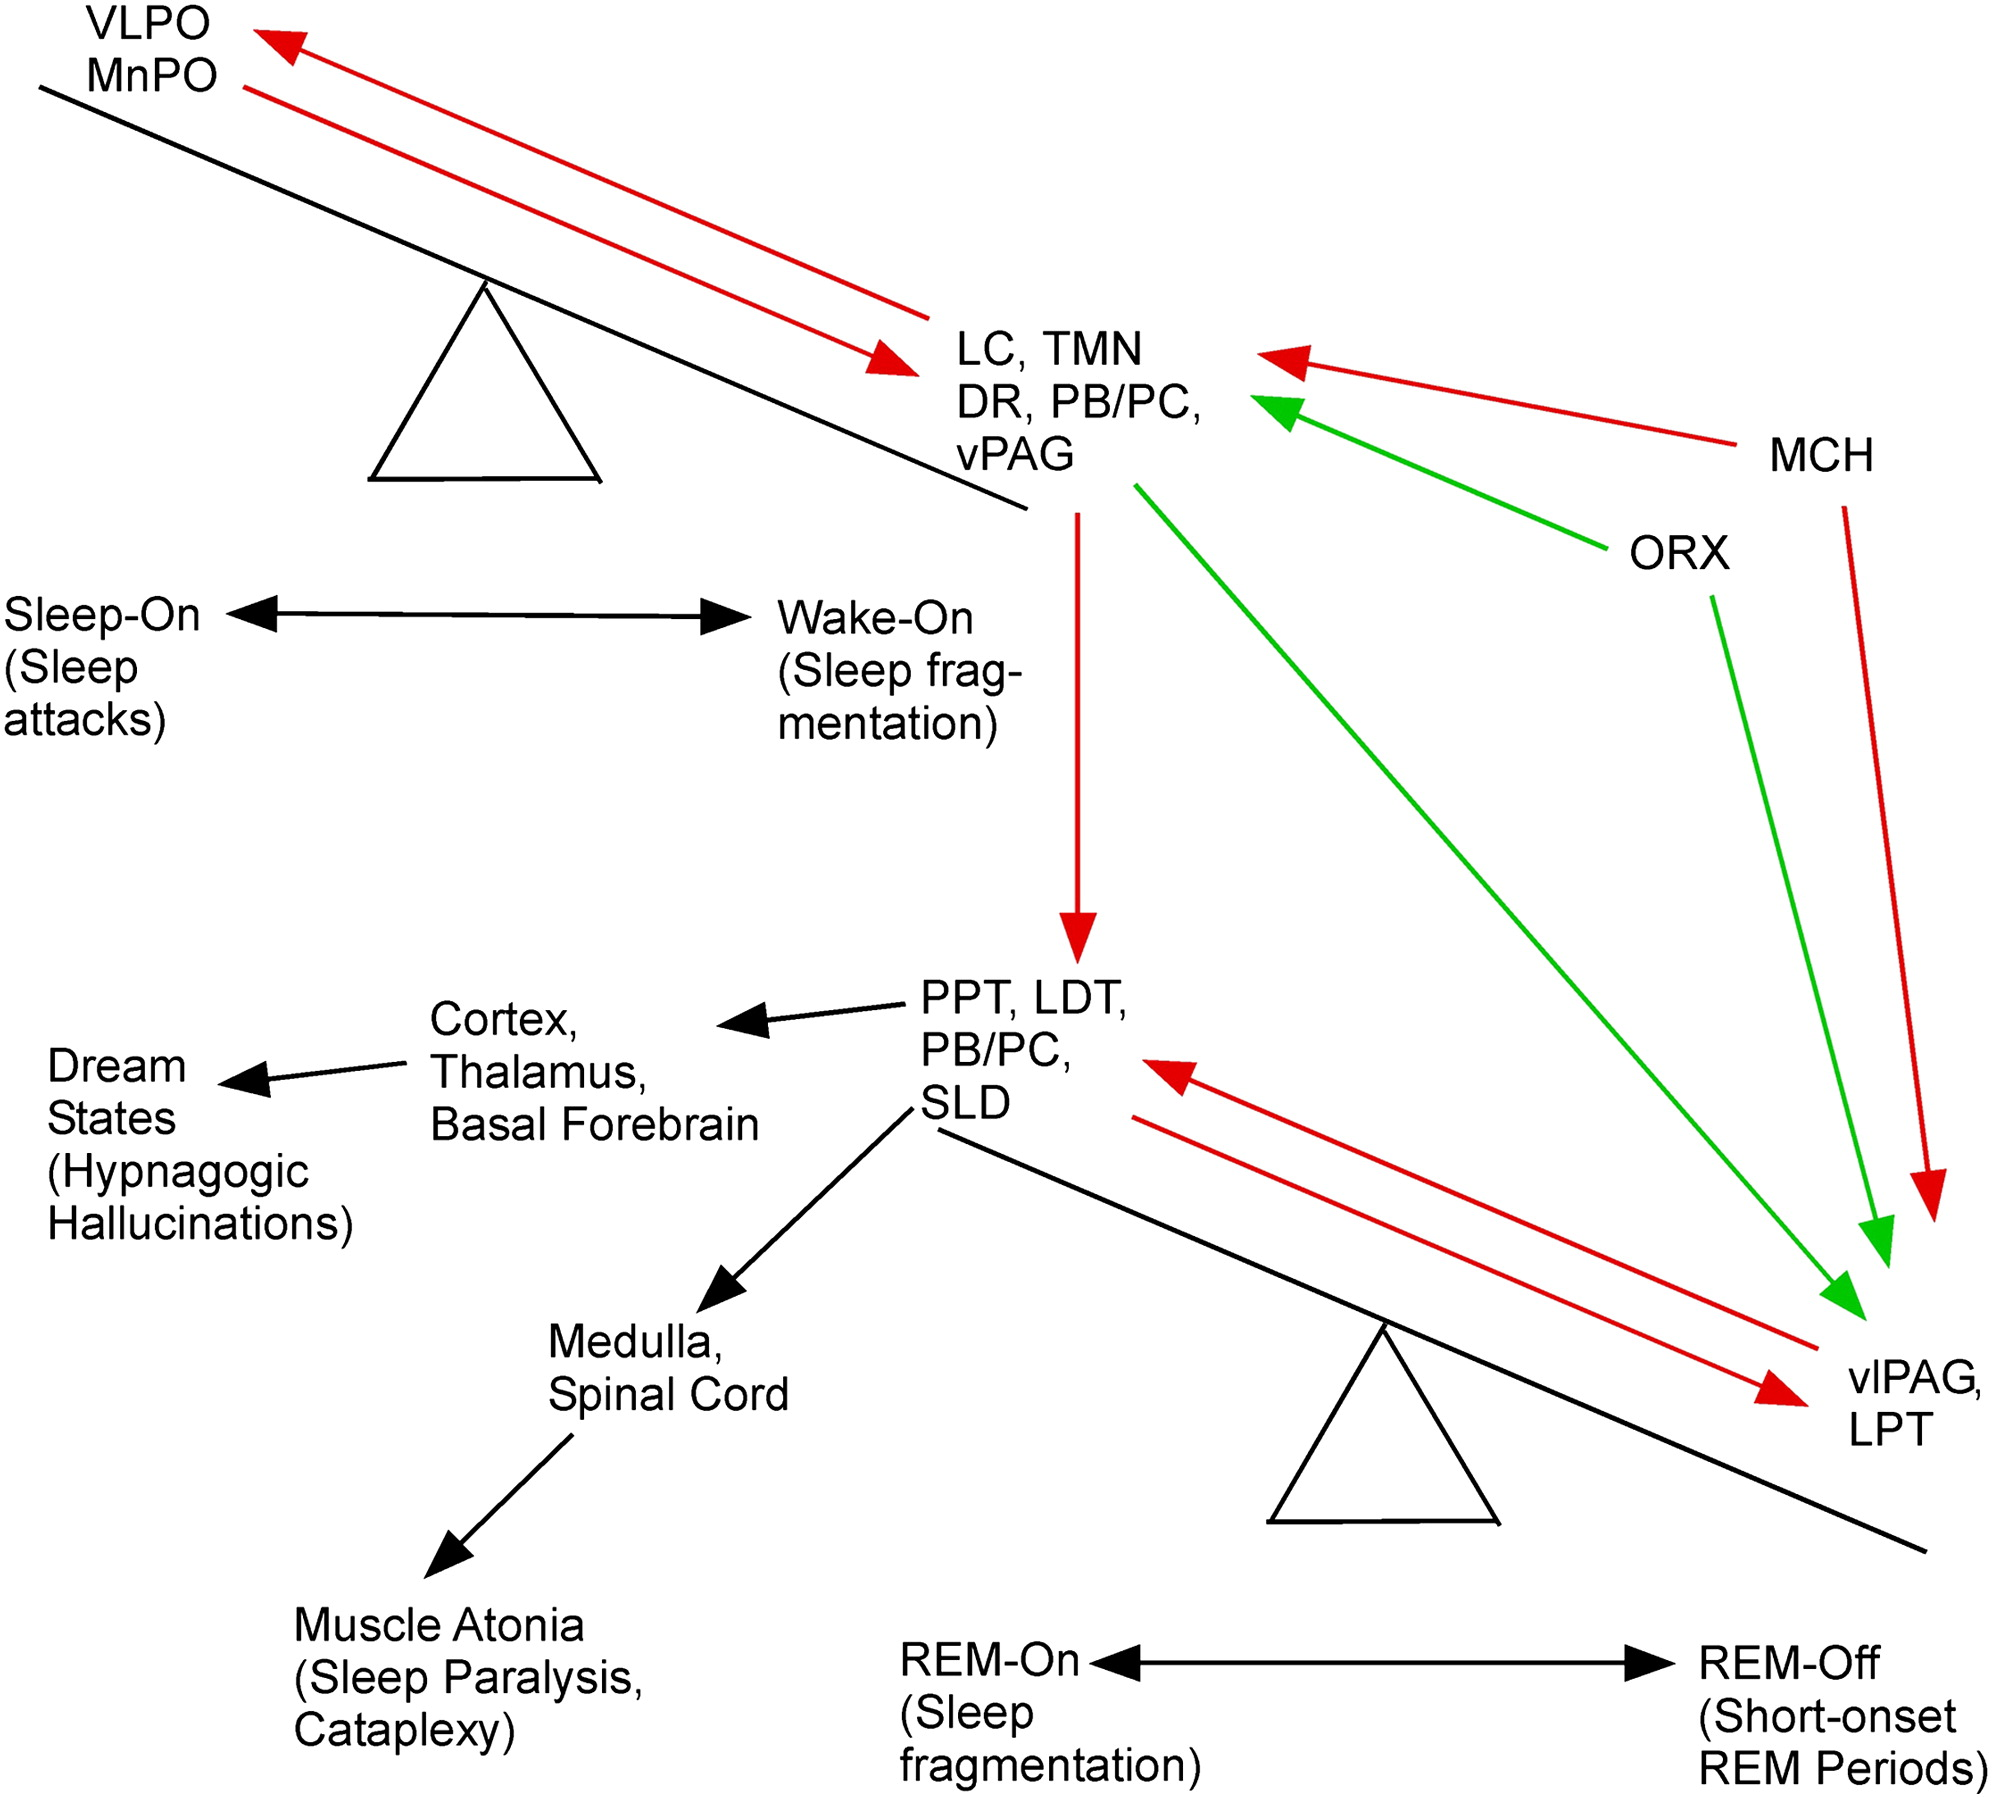
\includegraphics[width=\textwidth]{figures/clinical-background/SleepStateSwitching/Figure5.png}
                \caption[Schematic of the flip-flop model]{Schematic of the flip-flop model. Clinical manifestations of wrongful firing of neurons are shown in parentheses. %
                {\scriptsize{DR}}: dorsal raphe; %
                \describe{MnPO}; %
                \describe{LC}; %
                \describe{LDT}; %
                \describe{LPT}; %
                \describe{MCH}; %
                \textsc{orx}: orexin (hypocretin); %
                \describe{PB}; %
                \describe{PC}; %
                \describe{PPT}; %
                \describe{SLD}; %
                \describe{TMN}; %
                \describe{vlPAG}; %
                \describe{VLPO}; %
                \describe{vPAG}. %
                Reprinted from~\cite{Saper2010} with permission from Elsevier.}
                \label{fig:clinical-background:flipflop}
            \end{figure}
            
            It can be appreciated from the previous sections, that sleep and wake states are under the regulation of extremely complex mechanisms in the brainstem, thalamus, hypothalamus, and forebrain.
            These mechanisms can be grouped into the wake-sleep and \ac{REM}-\ac{NREM} promoting networks, which, in turn, can be combined into the \textit{flip-flop} model of sleep regulation~\cite{Saper2001, Saper2005, Saper2010}.
            
            A schematic shown in~\cref{fig:clinical-background:flipflop} illustrates both the complex neuronal interplay, as well as how two neurotransmitters play crucial roles in sleep homeostasis.
            One is the neuropeptide hypocretin, which acts to inhibit \ac{REM} entry by exciting the wake-promoting pathways and the \ac{REM}-off nuclei, while \ac{MCH} has the opposite effect of hypocretin.
            
            Also shown in~\cref{fig:clinical-background:flipflop} are clinical manifestations (in parentheses) associated with destabilized switching due to a lack of hypocretin\graffito{Lack of hypocretin-producing neurons is the hallmark sign of \ac{NT1}.}.
            
        \subsection{Micro-events durings sleep}\label{sec:sleep-events}
            \subsubsection{Arousals}
            Arousals are defined as abrupt shifts in \ac{EEG} frequencies towards alpha, theta, and beta rhythms for at least \SI{3}{\second} with a preceding period of stable sleep of at least \SI{10}{\second}.
            During \ac{REM} sleep, where the background \ac{EEG} shows similar rhythms, arousal scoring requires a concurrent increase in chin \ac{EMG} lasting at least \SI{1}{\second}.
                \citep{Ermis2010}
            \subsubsection{Movements of the extremities}
            \Acp{LM} should be scored in the leg \ac{EMG} channels, when there is an increase in amplitude of at least \SI{8}{\micro\volt} above baseline level with a duration between \SIrange{0.5}{10}{\second}.
            A \ac{PLM} series is then defined as a sequence of 4 \acp{LM}, where the time between \ac{LM} onsets is between \SIrange{5}{90}{\minute}.
            \subsubsection{Respiratory disturbances}
            Apneas are generally scored when there is a complete (\SI{>=90}{\percent} of pre-event baseline) cessation of breathing activity either due to a physical obstruction (obstructive apnea) or due to an underlying disruption in the central nervous system control (central apnea) for at least \SI{10}{\second}.
            When the breathing is only partially reduced (\SI{>=30}{\percent} of pre-event baseline) and the duration of the excursion is \SI{>=10}{\second}, the event is scored as a hypopnea if there is either a \SI{>=4}{\percent} oxygen desaturation or a \SI{>=3}{\percent} oxygen desaturation coupled with an \ac{Ar}.
            % \subsubsection{K-complexes and sleep spindles}
            %     \citep{Cash2009, Gennaro2003, Forget2011}
                
                
    \section{Recording and quantifying sleep}\label{sec:recording-quantifying-sleep}
    
        \subsection{Polysomnography}\label{sec:polysomnography}
            The principal tool available to sleep physicians and technicians for analysis of sleep patterns is the \textit{polysomnography} (\acs{PSG}).
            This is often the first study performed on patients referred to a sleep clinic, and consists of the continuous and concurrent recording of several physiological variables as electrophysiological signals.
            The primary signals of interest are brain activity (\ac{EEG}), eye movements (\ac{EOG}), chin and leg muscle activity (\ac{EMG}), heart activity (\ac{ECG}), respiratory effort (thoracoabdominal inductance plethysmography belts, RIP), nasal pressure, oral airflow, and blood oxygen saturation (pulse oximetry).
            Sleep experts manually analyze the contents of these signals in order to score sleep stages and annotate sleep events based on a standardized set of guidelines published by the \ac{AASM}~\cite{Berry2020}. 
            These guidelines also contain technical recommendations for recording sleep studies, such as electrode placements, minimal sampling frequencies and specific filter settings. \cref{tab:aasm_recordings} lists an overview of technical specifications for commonly recorded signals as recommended by the \ac{AASM}.
            
            \begin{figure}
            \begin{adjustwidth*}{}{-\marginparwidth-\marginparsep}
                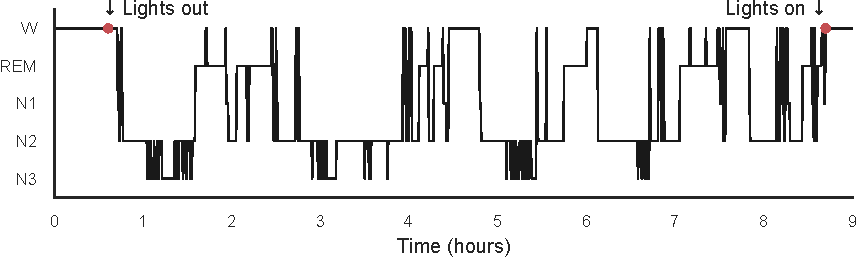
\includegraphics[width=\textwidth+\marginparwidth+\marginparsep]{figures/clinical-background/hypnogram.pdf}
                \caption[Hypnogram example of male subject]{Example of a hypnogram from a \acs{PSG} study of an 82 year old male subject.}
                \label{fig:clinical-background_hypnogram}
            \end{adjustwidth*}
            \end{figure}
            
            A common procedure for analysis of sleep studies involves multiple passes through each PSG study.
            For example, a first pass could be to score every consecutive segment of \SI{30}{\second} data as one of the five sleep stages.
            A second pass could be to score respiratory events, arousals and leg movements, etc. 
            The product of these passes is a sleep study report, which summarizes the findings into a hypnogram and associated PSG variables, including total sleep time (TST), sleep latency (SL), REM latency (RL), wake after sleep onset (WASO), and percentage of time spent in the different sleep stages.
            Key indices describing the amount of sleep events are also calculated for each study, such as the arousal index (number of arousals per hour of sleep, ArI), apnea-hypopnea index (number of apneas and hypopneas per hour of sleep, AHI), and the periodic limb movements in sleep index (number of peridoc limb movement series in sleep per hour of sleep, PLMSI). 

            \begin{table}[tb]
                \small
                \centering
                \caption[Technical specifications for recording \acs{PSG} signals]{Technical specifications for recording commong signals in \acsp{PSG} according to \acs{AASM}2020 standards~\cite{Berry2020}.}% used for subsequent visualization and analysis}
                \label{tab:aasm_recordings}
            \begin{threeparttable}
                \begin{tabular}{@{}llll@{}} \toprule
                    \textbf{Signal} & \textbf{Recommended recording setup} & \textbf{Min.} \(\mathbf{f_s}\) & \textbf{Filter} \\ \midrule
                    EEG & F4-M1, C4-M1, O2-M1 (required)    & \SI{200}{\hertz}  & \SIrange[range-units=single,range-phrase=--]{0.3}{35}{\hertz} \\
                        & F3-M2, C3-M2, O1-M2 (backup)      &                   &                                                               \\
                    EOG & E1-M2, E2-M2 (required)   & \SI{200}{\hertz}  & \SIrange[range-units=single,range-phrase=--]{0.3}{35}{\hertz} \\
                        & E1-M1, E2-M1 (backup)     &                   &                                                               \\
                    EMG & Chin2-ChinZ (required, chin EMG)  & \SI{200}{\hertz}  & \SIrange[range-units=single,range-phrase=--]{10}{100}{\hertz} \\
                        & Chin1-ChinZ (backup, chin EMG)    &                   &                                                               \\
                        & Bipolar derivation (required, leg EMG) & &                                            \\
                    ECG & modified Lead II derivation (required) & \SI{200}{\hertz} & \SIrange[range-units=single,range-phrase=--]{0.3}{70}{\hertz} \\ \bottomrule
                    % RIP & --- & \SI{25}{\hertz} & \SIrange[range-units=single,range-phrase=--]{0.1}{15}{\hertz} \\ 
                    % Nasal pressure & --- & \SI{25}{\hertz} & \SIrange[range-units=single,range-phrase=--]{\leq 0.03}{100}{\hertz} \\ 
                    % Airflow & --- & \SI{25}{\hertz} & \SIrange[range-units=single,range-phrase=--]{0.1}{15}{\hertz} \\ 
                    % Oximetry & --- & \SI{10}{\hertz} & \SIrange[range-units=single,range-phrase=--]{}{15}{\hertz} \\ \bottomrule
                \end{tabular}
            \begin{tablenotes}
            \item  \acs{AASM} describes a specific requirement as well as a backup in case of failure for each signal. Minimal \( f_s \) lists the minimally acceptable sampling frequency per signal, but the recommendations are higher in order to better capture waveform morphology. Filter settings describe recommended bandpass filter settings.
            \end{tablenotes}
            \end{threeparttable}
            \end{table}
            
        % \subsection{Multiple sleep latency test}
        % \subsection{Technical considerations when recording sleep studies}
    % \section{Abnormal sleep and sleep disorders}
        
    %     In the following sections are briefly described some of the common sleep disorders that are relevant to the topic of this thesis.
    %     % A diagnosis of sleep disorders is based on multiple parameters.
    %     Commonly, a patient is submitted to a sleep clinic under suspicion of a sleep disorder under referral from a general practitioner or physician, when they experience extreme tiredness during daylight hours, or perhaps a significant other experience nightly disturbances.
    %     Healthcare professionals make a diagnosis from the medical history, answers to questionnaires, findings from the PSG and/or MSLT, and lab test results, according to diagnostic criteria published by the AASM in~\citetitle{AASM2014}~\cite{AASM2014}.
        
    %     \subsection{Sleep related breathing disorders}
    %     Sleep disordered breathing comprise several disorders and syndromes, but is generally characterized by respiratory problems during sleep and sometimes during wakefulness.
        
    %     \textbf{Obstructive sleep apnea} (OSA) is characterized by recurrent restrictions in the upper airways~\cite{Malhotra2002}.
    %     It is a very common disease with \SIrange[range-units=single,range-phrase=--]{5}{15}{\percent} of the general population in the USA affected by OSA~\cite{Young}. 
        
    %     \subsection{Movement disorders}
        
    %     \subsection{Narcolepsy}
    
    %     \citep{AASM2014}
    \section{Challenges in scoring sleep studies}\label{sec:challenges-scoring-sleep-studies}
        Significant human bias can enter into the analysis of sleep studies by virtue of the process being performed manually.
        Several studies have shown significant \textit{inter-} and \textit{intra-}rater variability\graffito{Interrater variability refers to the variation in scoring that happens between experts on the same study, while intrarater variability refers to the variability in scoring when a single expert scores the same study more than once.} primarily in the case of sleep stage scoring, but some studies have also investigated the reliability of scoring arousals and respiratory events for sleep-related breathing disorders.
        This variability can be caused by several factors:
        \begin{enumerate}
            \item \textit{Imprecise scoring guidelines.}
            Some have argued that extensive training is required to minimize the subjective component in sleep stage scoring, and that the optimal training requires participation in concensus scoring rounds~\cite{Penzel2013}.
            \item \textit{Presence of disease or other sleep disorders.}
            Many neurodegenerative diseases exhibit symptoms of disturbed sleep as the neurodegeneration progresses to the centers in the brain stem responsible for control of sleep and wakefulness~\cite{Santamaria2011}.
            Similarly, central hypersomnias\graffito{Central disorders of hypersomnolence, \emph{hypersomnias}, are a group of sleep disorders characterized by excessive daytime sleepiness not caused by disturbed nocturnal sleep or irregular circadian rhythms~\cite{AmericanAcademyofSleepMedicine2014}} can also exhibit fragmented sleep.
            \ac{NT1}, for instance, shows increased fragmentation of sleep, because the hypocretin-producing cells in the latero-posterior hypothalamus responsible for stabilizing the wake-sleep and \ac{REM}-\ac{NREM} pathways are missing~\cite{Kornum2017}.
            Since current scoring guidelines are based on clinical experience in healthy subjects exhibiting normal sleep patterns, the scoring of sleep patterns becomes more difficult in this context.
            \item \textit{True errors.}
            These can occur when annotations are correctly made, but entered wrongly into a computer system or report. 
            However, these types of errors are difficult to measure in practice.
        \end{enumerate}
        
        A separate, but equally critical issue in scoring sleep studies concerns recording of the study itself by means of electrical equipment.
        Typically, the \ac{PSG} is performed as described in \cref{sec:polysomnography} with many electrodes placed on the body to the discomfort of the wearer potentially disrupting regular sleep patterns.
        For this reason, efforts are being made in industry and research to develop non-intrusive, low-impact recording devices, such as headbands, or in-ear \ac{EEG}~\cite{Mikkelsen2017,Mikkelsen2019}.
        
        Depending on the target variable under investigation, reliability and variability can be measured with different metrics.
        The following sections will describe some of the studies that have investigated inter- and intra-scorer reliability for various sleep analysis objectives.
        
        
        \subsection{Sleep stage scoring}\label{sec:challenges-sleep-stage-scoring}
        
            \citeauthor{Norman2000} found the average epoch by epoch agreement between five experienced PSG technicians representing different clinics to be \SI{73}{\percent} in a dataset containing 62 PSGs~\cite{Norman2000}.
            Furthermore, they also found this agreement to vary with phenotype, as the average agreement in a normal subset was higher than for a subset consisting of patients with sleep disordered breathing (\SI{76}{\percent} in the normal subset vs. \SI{71}{\percent} in the SDB subset).
            
            Later studies also found significant variability in expert agreements when comparing different patient groups. 
            Notably, \citeauthor{Danker-Hopfe2004} investigated interrater reliability between experienced technicians in eight different sleep clinics in Europe in a sample of 196 recordings from 98 patients exhibiting different disorders, such as depression, general anxiety disorder with and without insomnia, Parkinson's disease, sleep apnea and periodic leg movements in sleep disorder~\cite{Danker-Hopfe2004}.
            They found that although the overall agreement between experts as measured by \cohen{}\graffito{\cohen{} is a measure of the observed agreement between two agents taking into account chance agreement.} was \num{0.6816}, there was a statistically significant difference between patient groups, where the median $\kappa$ ranged from \num{0.6138} in patients with Parkinson's disease to \num{0.8176} in patients with generalized anxiety disorder.
            Other studies have found no statistically significant differences in the overall agreement between healthy controls, patients with sleep apnea/hypopnea syndrome, and patients with narcolepsy, when comparing scorers from Berlin and Beijing~\cite{Zhang2015a}. 
            They did, however, find statistically significant differences in the stage-specific agreements between patient groups.
            
            Recent large scale studies on interscorer agreement found that the average consensus-agreement is approximately \SI{83}{\percent} with the overall stage-specific agreement ranging from \SI{63}{\percent} for \ac{N1} to \SI{91}{\percent} for REM~\cite{Rosenberg2013}.
            Although the authors recognize that their results are heavily biased towards agreements in the \ac{N2} stage as this accounts for almost \SI{60}{\percent} of the total number of epochs, this percentage is in agreement with clinical experience and reflects the amount of \ac{N2} in a typical sleep study.
            
            Although human subjective bias is also a factor, the vast majority of interscorer differences originate from equivocal epochs that have equal probability of being assigned to two stages. 
            \citeauthor{Younes2016} found that disagreements were most common between \ac{W} and \ac{N1}, \ac{N2} and \ac{N3}, and \ac{N1} and \ac{N2}~\cite{Younes2016}, and indeed several studies have found that scoring \ac{N1} and \ac{N3} sleep is especially difficult~\cite{Danker-Hopfe2004,Rosenberg2013,Zhang2015a,Younes2018}.
            
        
        \subsection{Arousals}\label{sec:challenges-arousals}
        
            % While not as well described as scoring of sleep stages or respiratory events, some studies have been investigating the interscorer reliability for arousals.
            The majority of studies on reliability of arousal scoring are based on criteria from the \ac{ASDA}~\cite{Bonnet2007}.
            One study comparing several different criteria for arousal scoring found an \ac{ICC}\graffito{the intraclass correlation coefficient is a descriptive statistic for characterizing agreement between data that can be naturally organized in groups.} of 0.84 using the \ac{ASDA} criteria~\cite{Loredo1999}. 
            Experts scoring arousals shorter than \SI{3}{\second} with an \ac{ICC} between 0.19 and 0.37 were found less reliable, while the addition of increased \ac{EMG} activity as a criteria in addition to the \ac{ASDA} criteria increased the \ac{ICC} to 0.92.
            Another study, however, did not improve the already-high \ac{ICC} of 0.98 when supplementing the \ac{ASDA} criteria with increased \ac{EMG} activity~\cite{Smurra2001}.
            
            Another factor to be considered in the reliable scoring of arousals is the placement of the arousal in the sleep continuum.
            \citeauthor{Drinnan1998} investigated the impact of sleep stage on arousal scoring and found the highest \cohen value for arousals scored in slow wave sleep~\cite{Drinnan1998}.
            This sleep stage exhibits delta and \ac{SWA} \ac{EEG} rhythms with high amplitude and low frequency, which is easier to contrast with the shift to high frequency \ac{EEG} content typically associated with arousals.
            
            Other types of cues visible in the \ac{PSG} are the presence of autonomous findings such as increased heart rate visible in the \ac{ECG}, or increased respiratory effort.
            The latter is evident in a study investigating arousal scoring reliability in 17 \ac{OSA} patients using \ac{ASDA} criteria. 
            An event-by-event scoring agreement of \SI{91}{\percent}, which dropped significantly to \SI{59}{\percent} when removing the respiratory signals was found~\cite{Thomas2003}.
            
            While reliability of scoring arousals according to the updated \ac{AASM}2007 criteria remains severely understudied, \citeauthor{Magalang2013} reported an intraclass correlation coefficient for the arousal index of \muci{0.68}{0.49}{0.85} in 15 \acp{PSG} scored by nine technicians from unique sleep clinics according to \ac{AASM}2007 criteria~\cite{Magalang2013}.
            
            These reported results are based solely on the values of the arousal index per study, and as such, two scorers can potentially score completely different arousals for a specific \ac{PSG}, while still having good agreement between them, since their scored arousal index values are similar. 
            Furthermore, scoring only index values for a study do not reflect important underlying characteristics of the arousal events.
            These characteristics could include event morphology and variability in each recorded modality, as well as variations in duration, spectral content, amplitude, \etc.
            % The arousal index, as well as other index values commonly reported in the \ac{PSG} report, are only approximations of complex, dynamic process that involve multiple systems in the body.
            % Another issue 
           
            
            
        \subsection{Sleep disordered breathing}\label{sec:challenges-sdb}
        
            \citeauthor{Whitney1998} investigated inter- and intra-scorer reliability in three technicians for 20 randomly selected \ac{PSG} recordings from the \ac{SHHS} cohort using various definitions of \acp{RDI} with or without arousals, and oxygen desaturation levels from \SIrange{2}{5}{\percent}~\cite{Whitney1998}.
            The authors found that the technicians were in high agreement when scoring respiratory events with oxygen desaturation levels present indicated by an \ac{ICC} between 0.90 and 0.99.
            However, this reliability dropped to moderate agreement when oxygen levels were not part of the scoring (\ac{ICC} of 0.77), and when neither oxygen levels or arousals were included (\ac{ICC} of 0.74).
            
            The study by~\citeauthor{Magalang2013} also investigated the agreement in scoring respiratory events.
            The authors reported an \ac{ICC} for the \ac{AHI} of \muci{0.95}{0.91}{0.98} which indicates a very strong agreement between centers.
            
            \citeauthor{Rosenberg2014} studied the degree of agreement between more than \num{3600} scorers when asked to identify whether a \SI{30}{\second} epoch contained either an obstructive, mixed or central apnea; a hypopnea; or no event at all~\cite{Rosenberg2014}.
            They found that overall agreement was 93.3\%, although this was caused by a very high agreement of 97.4\% on epochs with no event present.
            For epochs with a majority vote of having a respiratory event present, overall agreement was 88.4\%.
            The study also showed that disagreements between apneas and hypopneas, and between different types of apneas were common.
            
            However, as with the arousal scoring, neither the \ac{RDI} nor the \ac{AHI} take into account the exact location of respiratory events, which means that two technicians in theory could be in perfect agreement when comparing these values even though they did not score any of the same events.
            
            % \citeauthor{Whitney1998}\citeyear{Whitney1998}\cite{Whitney1998}
            
            % \citeauthor{Magalang2013}\cite{Magalang2013}
            
            % \citeauthor{Rosenberg2014}\cite{Rosenberg2014}
        
        % Papers that discuss sleep stage scoring
        % \begin{itemize}
        %     \item \fullcite{Norman2000}
        %     \item \fullcite{Danker-Hopfe2009a}
        %     \item \fullcite{Rosenberg2013}
        %     \item \fullcite{Penzel2014}
        %     \item \fullcite{Zhang2015a}
        %     \item \fullcite{Younes2016}
        %     \item \fullcite{Younes2018}
        % \end{itemize}
        % Papers for sleep disordered breathing
        % \begin{itemize}
        %     \item \fullcite{Rosenberg2014}
        %     \item \fullcite{Magalang2013}
        %     \item \fullcite{Redline2007}
        % \end{itemize}
        % Papers for arousals
        % \begin{itemize}
        %     \item \fullcite{Magalang2013}
        %     \item \fullcite{Bonnet2007}
        % \end{itemize}
    \section{Chapter summary}
    
    This chapter has introduced some of the fundamental aspects in sleep science.
    
    The concepts of \textit{macro-} and \textit{micro-}sleep were introduced.
    The former was elaborated upon with descriptions of the five sleep stages%\graffito{\acf{W}, \acf{N1}, \acf{N2}, \acf{N3}, and \acf{REM}.} 
    currently recognized by the~\ac{AASM}, and how they together form a description of the sleep architecture called a hypnogram.
    
    The chapter described the neurobiological mechanisms and complex interplay between cell nuclei in the brainstem responsible for sleep regulation.
    For example, the wake-sleep and \ac{REM}-\ac{NREM} switches consist of several neuron groups in the basal forebrain, hypothalamic areas, and brainstem.
    Their mutual interactions responsible for the fast and complete transitions between wake and sleep, and \ac{REM}-on and \ac{REM}-off periods, can be conceptualized in the flip-flop model, which summarizes the roles of the different cell groups and neurotransmitter systems.
    
    Although, this chapter did not elaborate on various malfunctions of the sleep regulatory systems in the brainstem, later chapters will touch on specific sleep disorders where applicable, such as narcolepsy in~\cref{chap:classification-sleep-disorders}.
    
    The final sections in this chapter touched upon some of the issues facing clinical sleep medicine.
    Specifically, the reproducibility of scoring sleep studies, the intra- and inter-scorer reliability of scoring sleep stages, arousals, and sleep disordered breathing events were presented and discussed.
    The difficulty in providing accurate and reproducible results with clinical outcomes is specifically a motivating factor for this thesis; namely the development of robust systems to automatically process and analyze clinical sleep studies.
    